\chapter{State-of-the-Art}\label{chap:state-art}
In the demand for an effective, high-quality approach to the analysis of isolates from infected animals, molecular studies help to investigate characteristics of the sample. Genome analysis has become an integral part of animal disease surveillance, especially since the advent of high-throughput sequencing technologies in the last 15 years. Next-generation techniques and applications are described below, the state of the art in poxvirus and avian influenza virus detection and analysis, and lastly the drawbacks of the methods discussed.

\section{High-throughput Technologies in Diagnostic Virology}
When comparing DNA sequencing technologies, there are differences in speed, throughput and volume of sequences. The term ''next-generation'' in NGS used to describe newer technologies in the field implies a next step in the evolution of sequencing technologies. As sequencing machine technologies evolve rapidly, there are gradations such as ''second-generation'' and ''third-generation''. Following the original 1977 Sanger sequencing method using radioactivity and gels, second-generation sequencers are advancements of Sanger sequencing that uses sequencing by synthesis~\cite{mardis2008next}. In second-generation methods, reactions run in parallel and drastically reduce overall costs compared to Sanger sequencing. They produce short sequence reads length and are able to detect reads without using electrophoresis.
Third-generation sequencing technologies typically generate longer primary reads of DNA (and RNA) molecules while maintaining the massive parallelism of the technology and taking advantage of this benefit~\cite{slatko2018overview}. The nowadays most commonly used next-generation technologies for DNA sequencing and their applications are described below.

\subsection{Overview of NGS Platforms and Applications}
By far the biggest player in the field of DNA sequencing is the Illumina platform, first developed by Solexa and Lync Therapeutics~\cite{illumina2015introduction}. Illumina sequencing is based on bridge amplification, which creates clusters of copies of each DNA fragment. This technique involves repeated synthesis reactions with proprietary modified nucleotides containing a different fluorescent label for each of the four bases A, T, C and G. The reactions are performed over 300 or more rounds, and fluorescent detection allows for faster detection through direct imaging. An Illumina sequencer outputs data in the form of sequence reads, which are short DNA fragments ranging from 50 to 600 base pairs in length depending on the specific instrument and protocol used~\cite{illumina2015introduction, slatko2018overview, mardis2008next}. The output data from an Illumina sequencer typically is in the form of raw sequence files in FASTQ format, which contain the base calls and corresponding quality scores for each read. These reads can be used for downstream analyses such as viral genome assembly and variant calling.

Oxford Nanopore Technologies (ONT) is a third-generation paradigm shifting sequencing technology. It measures changes in ionic current accross membranes as single-stranded DNA nucleotides pass through a nanopore~\cite{jain2016oxford}. Nanopore-based DNA sequencing technologies are purchasable as a portable, small MinION (ONT) device, allowing experts to use it for applications where space requirements or portability are important~\cite{greninger2015rapid, jain2016oxford}. The cyclic mode of sequencing used in second-generation approaches is replaced by sequencing in real-time with read lengths of up to 10,000 basepairs~\cite{jain2016oxford}. Despite its advantages, the main caveat of ONT is its relatively high error rate compared to other HTS methods~\cite{fu2019comparative}. This makes ONT less suitable for single-nucleotide variant analysis that is required in some diagnostic applications~\cite{bowden2019sequencing, stefan2022comparison}.

Other frequently used second-generation platforms are Roche/454 sequencing, Ion Torrent (Thermo Fisher) technology and SOLiD (Sequencing by Oligonucleotide Ligation and Detection). Third-generation platforms include single molecule real-time sequencing (SMRT) by PacBio and nanopore sequencing~\cite{rhoads2015pacbio}. 

\begin{figure}
	\centering
	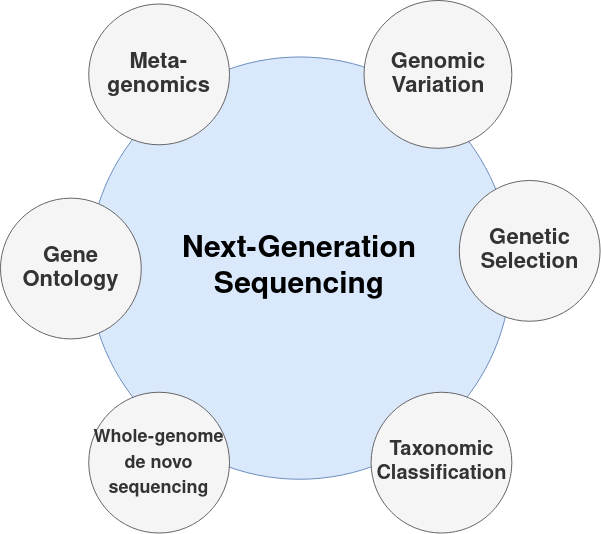
\includegraphics[width=0.5\textwidth]{media/2-ngs.png}
	\caption{Overview of next-generation sequencing technology applications in diagnostic virology.}
	\label{fig:2-ngs}
\end{figure} 

As NGS platforms are widely used in biomedical and clinical contexts, some of the most important applications in diagnostic virology are depicted in Figure~\ref{fig:2-ngs}. In virology, metagenomics can be used to identify viruses in complex clinical samples~\cite{chiu2019clinical}. It allows for the detection of known and novel viruses without prior knowledge of the infectious agent. Metagenomics involves the sequencing of all genetic material in a sample, including viral genomes, to identify the presence of viruses. Once a virus is identified, genomic variation refers to differences in the DNA sequence of a virus between different strains or isolates. These variations can be used for tracking the spread of an outbreak, identification of sources of an infection, or determination of the level of virus virulence~\cite{capobianchi2013next}. \\ 
Genetic selection describes to the process by which certain viral strains become more prevalent in a population over time due to selective pressures. In diagnostic virology, genetic selection is used to track the evolution of a virus in the course of time and determine which strains are most likely to cause outbreaks or epidemics. This is of special interest in the backtracing of infected animals to know where the virus came from. Using gene ontology, functions and interactions of genes are described. This is crucial to identify the genes responsible for specific viral functions and to understand how these functions contribute to viral pathogenesis. \\
Based on their genetic and structural characteristics, viruses are classified to existing systems, called taxonomic classification. This clustering analysis can be used for the type identification of a virus causing infections and determination of its potential for transmission and pathogenicity~\cite{dutilh2021perspective}.\\
Whole-genome de novo sequencing is the sequencing of an entire viral genome without prior knowledge of its genetic sequence. Similar to metagenomics, this technique can be used to identify novel viruses, to study mutations in viral genomes and to track the evolution of a virus over time~\cite{slatko2018overview}.

\subsection{Detection of Viral Pathogens}
For NGS methods to be a viable tool in diagnosis of viral animal diseases, the methods must be efficient and reliable. Almost all downstream analyses depend on the data obtained by sequencing, so it is imperative to choose the most appropriate method for each application. Metagenomics-based approaches use whole-genome sequencing to characterise viral diversity in animal, human and environmental samples. The detection of rare and novel infectious pathogens and the study of mutations in the genome are crucial for developing a deeper understanding of livestock viromes and potential zoonotic agents. In addition, NGS has been shown to detect non-culturable organisms as well as co-infections that have not been detected using traditional microbiological approaches~\cite{cantalupo2019detecting}. Metagenome sequencing often relies on a low number of pathogenic reads to detect and to make diagnostic calls. As sequencing depth directly influences genome coverage that can be obtained, the optimal amount of data to cover the complete genome is necessary. It has been shown that for a full virus genome to be represented, NGS data generated from ribo-depleted total RNA with a minimum length of one million high-quality reads works best~\cite{visser2016next}. Nevertheless, validation pipelines and confirmatory tests are needed for NGS approaches to pathogen detection~\cite{minogue2019next}.
\todo{more?}

% WOAH/FAO: Network of Expertise on Animal Influenza
% WHO: GISRS (Global Influenza Surveillance and Response System) for human influenza,
% WHO: FluNet
% WHO: GISAID (Global Initiative on Sharing All Influenza Data)
% \cite{daniels2023health}

\subsection{Data Analysis Issues}
Since the surveillance of viral animal diseases with NGS is advancing rapidly, it is important that regions and health organizations that experience high damage of viral outbreaks but do not have their own facilities and know-how have access to the needed tools and knowledge. Costs for NGS sequencers are still high and the access to appropriate laboratories is not given everywhere. Networks like VETLAB and standardisation of techniques, for example freely available and published by the WOAH, can enable professionals worldwide independent of their equipment on site. In the scope of the ZODIAC project, this aspect is addressed by providing protocols for each step from taking samples of potentially infected animals to the detailed analysis and derived actions~\cite{zodiac2021}.\\
This emphasizes the importance of free and easy-access platforms that entitle professionals to analyse their samples. Technical know-how to develop and maintain servers for analysis of NGS data is not part of the average global standard tool package, even though multidisciplinary approaches can help to facilitate by being shared through platforms.

NGS methods themselves have downsides that need to be considered when applying these techniques. Generally, chimerical sequences are formed during sequencing, which may be interpreted as false positives for novel organisms. Chimeric products are artifacts originating from joining sequences and are represented by point mutations, insertions and deletions. Chimera formation also occurs during PCR amplification~\cite{zylstra1998pcr}.\\
During bioinformatics analysis steps using algorithms with computationally expensive steps, the choice of the algorithm as well as its configuration settings have huge impact on the final results obtained. This includes algorithms in steps such as filtering for quality, clustering and sequence classification~\cite{kopylova2016open}. The cleaning step or filtering phase eliminates low-quality reads from the dataset, whereas the error correction process distinguishes true variants from those caused by experimental noise. This is based on the concept that errors occur randomly with low frequency, while true mutations tend to be clustered, and their frequency can be measured~\cite{zagordi2010error}. Longer reads avoid this problem because contigs must not be assembled in the first place, avoiding clustering and filtering errors. This is why the shift in third-generation and later sequencing platforms is towards longer reads again. \\
Each application of software with NGS data requires expertise in resolving limitations and drawbacks of specific methods. This in turn requires skills and experience in the field and the careful interpretation of results. Still, NGS provides a large pool of methods which eases this task, although available algorithms for genome assembly and amplicon analysis have drawbacks and limitations~\cite{finotello2012comparative}.

\section{NGS Methods for Poxviruses}
In the following, current approaches to analyse NGS data of poxviruses are described. To get into the topic, the characteristics of poxviruses are examined.

\subsection{Poxviruses}
Throughout human history, poxviruses have played a significant role with variola being the most notorious as it is the causative agent of smallpox. Smallpox has been described in Chinese texts dating back to the 4th Century AD, and evidence of pox-like scars found on Egyptian mummies suggests the disease may have existed as far back as the 2nd millennium BC~\cite{fenner1988history}. The discovery of a vaccine for smallpox made it the first disease to be eradicated by human efforts, and variola was the first human virus to be successfully eliminated~\cite{fenner2000adventures}. Modern vaccinology owes its origins to Edward Jenner's discovery in the late 18th century that zoonotic infections with the ''cowpox virus'' provided immunity to smallpox~\cite{fenner1988history}. Furthermore, vaccinia virus, which is now used for smallpox vaccination, was the first animal virus to be observed using electron microscopy and the first to be utilized as a vector for transporting foreign genes into animals. This is why poxviruses are among the best-known viruses. \\
The family of poxviruses, \textit{Poxviridae}, is a family of double-stranded DNA viruses. Its natural hosts are vertebrates and arthropods and there are currently 83 species within 22 genera in this family. The family is divided into two subfamilies, \textit{Entemopoxvirinae} (insect-infecting viruses) and \textit{Chordopoxvirinae} (vertebrate-infecting viruses). \\
Historically, poxviruses were classified based on disease symptoms and the animal species that was infected. Humans, cows, sheep, goats, horses and pigs have been studied to determine not only clinical symptoms but with the aim to classify poxviruses. This genus classisification has been confirmed by recent comparative genome analysis~\cite{gubser2004poxvirus}. Symptoms of disease caused by a poxvirus infection are skin lesions that can differ in size. Depending on the type of poxvirus, the papules can vary from small and pearly papules in infections of lumpy skin disease virus (LSDV) to larger crusts and spread generalized pustules in infections with the variola virus. Other general symptoms include fever, headache and rash.

\renewcommand{\arraystretch}{1.4}
\begin{table}[ht!]
	\begin{tabular}{lll}
	\hline
	\textbf{Genus}      & \textbf{Virus Species}                          & \textbf{Natural Hosts}                      \\ \hline
	Avipoxvirus         & Canarypox virus                                 & Songbirds 									\\ 
						& Fowlpox virus                                   & Chickens, turkeys                           \\ \hline
	Capripoxvirus       & Sheep pox virus                                 & Sheep                                       \\
	                    & Lumpy skin disease virus                        & Cattle                                      \\ \hline
	Centapoxvirus       & Yokapox virus\textsuperscript{1}                & Humans, mosquitoes                          \\ \hline
	Cervidpoxvirus      & Deerpox virus                                   & Deer                                        \\ \hline
	Crocodylidpoxvirus  & Crocodilepox virus                              & Crocodiles                                  \\ \hline
	Leporipoxvirus      & Myxoma virus                                    & Rabbits, hares                              \\ \hline
	Molluscipoxvirus    & Molluscum contagiosum virus\textsuperscript{1}  & Humans, primates, birds, dogs               \\ \hline
	Orthopoxvirus       & Variola virus (Smallpox)                        & Humans (eradicated)                         \\ 
						& Mpox virus\textsuperscript{1}                   & Humans, primates                            \\ 
						& Cowpox virus\textsuperscript{1}                 & Humans, cats, cows, elephants               \\ 
						& Vaccinia virus\textsuperscript{1}               & Humans, cattle, buffalos, rabbits           \\ 
						& Camelpox virus                                  & Camels                                      \\ \hline
	Parapoxvirus        & Pseudocowpox virus\textsuperscript{1}           & Humans, cattle                              \\ 
						& Orf virus\textsuperscript{1}                    & Humans, sheep, goats, etc.                  \\ \hline
	Suipoxvirus         & Swinepox virus                                  & Pigs                                        \\ \hline
	Yatapoxvirus        & Yaba monkey tumour virus\textsuperscript{1}     & Humans, rhesus monkeys                      \\ \hline
	\textsuperscript{1} Zoonotic disease &                                &                                             \\
	\end{tabular}
	\caption{Representative viruses from ten Chordopoxvirus genera.}
	\label{tab:2-chordopox}
\end{table}

Table~\ref{tab:2-chordopox} shows ten representatives of the 18 Chordopoxvirus genera according to the newest ICTV (International Committee on Taxonomy of Viruses) Taxonomy Release from 2021, while at least five genera contain zoonotic poxviruses~\cite{tax2021pox}. Orthopoxviruses have the biggest impact on human and animal health, and are remarkable for their broad host spectrum ranging from humans to wild and domestic animals~\cite{fenner2000adventures}.
The Chordopoxvirus subfamily is characterised by its large, linear double-stranded genome. Size varies between 134 to 365 kilobases~\cite{brunetti2003complete, tulman2004genome}. Chordopoxvirus genomes contain 130 to 328 open reading frames (ORF), and typically, two identical inverted terminal repeats (ITR) are located at both ends of poxvirus genomes. \\
Vaccination is available for smallpox, and the vaccine is even considered protective against symptoms of all orthopoxvirus infections. It is recommended for laboratory staff that works with mpox, cowpox, vaccinia and variola~\cite{cono2003smallpox}. For animals, there is a smallpox-based vaccine that is used to protect elephants against cowpox~\cite{kurth2008rat}. Sheep and goats are broadly vaccinated with an orf vaccine, which is, similar to smallpox vaccine, a live virus. The effective vaccination against existing poxvirus diseases and further microbiological studies, as well as similarities between poxviruses, motivate the expansion of existing data analysis pipelines that work for a specific poxvirus so that they can also work with other poxviruses.

\subsubsection*{Lumpy Skin Disease Virus}
Lumpy Skin Disease is caused by the lumpy skin disease virus belonging to the \textit{Capripoxvirus} (CaPV) genus within the family of poxviruses, subfamily \textit{Chordopoxvirinae}~\cite{walker2019changes}. The LSD virus genome is a double-stranded linear DNA molecule of circa 151 kilobasepairs in length. It contains between 147 and 156 open reading frames. Similar to other poxviruses, the LSDV genome consists of a central coding region which is bounded by two identical ITR regions with a length of circa 2,400 basepairs at both ends of the genome. This is a key characteristic to consider during reconstruction of the genome. With a sequence identity of over 96\% with the other CaPV genus members sheep pox and goatpox, the LSDV genome is highly similar to the other CaPV genomes~\cite{tulman2001genome}. \\
LSDV is not known to be transmissiable to humans and therefore not a zoonosis. Natural hosts of LSDV are cattle and Asian water buffalos. Although CaPV is considered to be host specific, sheep pox and goatpox strains can naturally cross-infect in both host species. There have been no cases of natural infection of sheep or goats with LSDV reported~\cite{namazi2021lumpy}. The three CaPV viruses are the most serious poxvirus diseases of livestock in terms of economic losses in the case of an outbreak. \\
Cattle infected with the LSDV typically show symptoms like fever, reduced feed and water uptake and characteristic skin nodules. The number of lesions varies from a few to many, covering the whole body~\cite{prozesky1982study}. From these symptoms alone, it is impossible to differentiate the diagnosis between sheep pox, goatpox and lumpy skin disease. Even with classical methods like cell culture and electron microscopy the highly similar viruses cannot be distinguished. Nowadays, polymerase chain reaction (PCR) and sequencing are the techniques used to provide the sensitive detection of CaPv~\cite{lafar2020capripoxvirus}.

LSDV has spread from the African continent and since 2019 reached major cattle producer countries in Asia, mainly India, Republic of China and Bangladesh. Other bigger outbreaks in south-west Europe were reported in 2014 to 2018, although these countries opted for a strict vaccination program and successfully eliminated LSDV from the region~\cite{prevention2017control}. In African and Asian countries, veterinarians struggle to fight endemic LSDV outbreaks because of a lacking financial support by governments, justified by low mortality and morbidity rates.

One strain of LSDV that has been extensively studied is the Neethling strain, first isolated in Kenya in 1958. It constitutes the strain used for the live attenuated vaccine that is widely used, if accessible, for cattle against LSDV outbreaks. Some countries use sheep pox vaccines to protect cattle against LSD, even though it does not bring complete immunity. Nevertheless they are used in regions where all CaPV are prevalent~\cite{brenner2009appearance}.

\subsection{Application of NGS Technologies in Poxvirus Diagnostics}
% GF-TADs in Europe
characteristic ITR that is left out in other pipelines (Yale University primer scheme starts after and ends before ITR)

https://www.sciencedirect.com/science/article/pii/S0166093422000118 explains Primer scheme and why tiling amplicon approach makes sense even for large genome size of CaPV genome and complex structure with repetitive ITR regions

* VirusDetect https://www.sciencedirect.com/science/article/pii/S0042682216303166
virus discovery using sRNA sequences. evaluates sRNA size profiles

* VirIdAl https://www.mdpi.com/1999-4915/13/10/2006
detecting and identifying viral pathogens in sequencing data. filtering, virus search (megablast), additional search

* with Neural-KSP \url{https://www.researchgate.net/publication/307615364_Finishing_monkeypox_genomes_from_short_reads_Assembly_analysis_and_a_neural_network_method}
monkeypox genome construction. "smart" gap filling


\section{NGS Methods for Avian Influenza Virus}\label{sec:AIV}
\subsection{Avian Influenza Virus}
Informally known as bird flu, avian influenza is a viral infectious disease that affects wild birds and poultry. The avian influenza virus (AIV) has occasionally crossed the species barrier and infects mammals, including humans. This makes it a high-priority zoonotic viral disease that has been designated as notifiable by WHO and WOAH~\cite{woah2023list}. Avian influenza occurs in two variants determining its severity: low pathogenic avian influenza (LPAI) and high pathogenic avian influenza (HPAI), although only HPAI cases need to be reported. The virus indirectly spreads through contaminated material, e.g. through feed, water supplies, feces or feathers. It directly spreads bird-to-bird via airborne transmission, and mainly through the overregional movement of wild birds as via bird migration over longer distances. Humans are infected through close contact with infected livestock or wild birds, and most reported infections of avian influenza in humans come from farm workers and others who are exposed in markets, production or clinical contexts~\cite{webster1992evolution}. \\
Symptoms of severe illness are characterised by influenza-like signs such as fever, nasal discharge, coughing and conjunctivitis. This holds for infections in both human and mammals infections, while infected birds show signs of swollen heads, lack of appetite, respiratory breathing difficulties and a drop in egg production.

AIV contains a negative-sense, single-stranded segmented RNA genome, so co-infection can lead to reassortment events. Avian influenza viruses are members of the \textit{Orthomyxoviridae} family and the four types Influenza A, B, C and D are distinguished on the basis of the presence of the nucleoprotein (NP) and matrix (M1) proteins~\cite{webster1992evolution}. AIV subtypes are determined by the hemagglutinin (HA) and neuraminidase (NA) segments, which include all known influenza A virus subtypes H1-H16 in combination with N1-N11~\cite{webster1992evolution, krammer2018influenza}. In order to be infectious, a virus particle has to contain each of the eight unique segments PB2 (poymerase), PB1/PB1-F2 (polymerase), PA/PA-X (polymerase), HA, NP, NA, M1/M2 and NS1/NEP (distinct non-strucutral proteins). Mutations in the HA and NA genes occur relatively frequently due to the prone-error RNA polymerase in the viral genome. AIV subtypes H5 and H7 of LPAI usually infect poultry, although the natural hosts of avian influenza A are wild waterfowl. These subtypes can change to a HPAI during circulation in poultry stocks by recombination with other gene segments or host genome~\cite{webster2006h5n1}. Both LPAI and HPAI infections have been reported in domestic poultry, i.e. ducks and chickens, turkeys, caged birds, aquatic birds and wild birds. \\
The H5, H7 and H9 subtypes are responsible for the biggest outbreaks of AIV with human cases~\cite{widdowson2017global}. The first confirmed report of human infection with an animal avian influenza virus dates 1958, and since then 16 subtypes have been found in humans~\cite{kluska1961demonstration}. Zoonotic spillover events have occurred with increasing frequency since the beginning of the 20th century and caused major endemics such as a huge H5 outbreak in the U.S. in 2014-2015, which led to over 25 million dead birds~\cite{seeger2021poultry}. Another ongoing outbreak that led to more than 58 million dead birds and costs of roughly 661 million U.S. dollars started in 2022 and spreads in the U.S.~\cite{usda2023hpai}. 
To defend avian influenza, vaccination against HPAI in poultry are widely used in China, Egypt, Indonesia and Vietnam. It also works as a preventive tool in the case of an outbreak to reduce the risk of introduction of the virus to poultry populations~\cite{swayne2013current, swayne2011assessment}. 

\subsection{Application of NGS Technologies in Avian Influenza Virus Diagnostics}
surveillance systems include classical phylogenetic methods to genotype novel emerging strains, classify viral lineages or assess tree topologies to distinguish between novel and emerging strains (taxonomic classification -- there are many strains)
%%%%%
SARS-CoV-2 tracking is of huge global interest, resulting in a highly regarded topic with ongoing scientific activity in terms of publications \\
includes established institutions in bioinformatics that hand out approaches, guidelines, recommendations to govern outbreaks of viral livestock diseases. includes comprehensive pipelines for bioinformaticians, veterinarians and other health professionals.
major platforms that offer exhaustive approaches to analyse genomic samples from infected stock. \\

INSaFLU, ViReflow? (SARS-CoV-2 samples) \\
 VAPOR (ref datasets) \\

* INSaFLU (inside the flu) -> for influenza, NGS towards metagenomic virus detection, routine genomic surveillance, 

* Nextstrain -> for RT SARS-CoV-2, Influenza, Ebola pathogen populations 
* Kraken2 -> taxonomic sequence classifier (using database and k-mers of FASTA sequences)
* VirFind (by Arkansas High Performance Computing Center) -> for fasta/Illumina fastq files, to detect new samples (trimming, mapping to ref, de novo assembly, Blastn, Blastx)
* ARTIC Network -> RAMPART for Ebola, yellow fever virus (read assignment, mapping, phylogenetic analysis on ONT data)
* IRIDA -> Integrated Rapid Infectious Disease Analysis for NGS data e.g. de novo assembly (FLAsh, SPAdes, Prokka)

tracking viruses using genomic sequence data collection; effective surveillance does not require exhaustive case surveillance, instead the collection of enough data from representative populations. This enables health professionals to detect newly evolved variants and to monitor trends in the circulating variants.\\
wastewater

https://synapse.koreamed.org/articles/1134050
